\section{Exercise 1}

Theo mạch mô phỏng trên (Hình 1.2), hãy xác định điện áp trên điện trở và diode ($V_R, V_D$), cũng như dòng điện I trong mạch với hai giá trị khác nhau của $R_1$, bao gồm 220 Ohm và 1,5K Ohm. Giả sử rằng mô hình diode hoàn chỉnh được sử dụng để phân tích, có điện áp thuận ở mức 0,7V và điện trở bên trong bằng 50 Ohm.

Cuối cùng, mô phỏng trên PSpice được chạy để kiểm tra lại với tính toán lý thuyết. Giải thích ngắn gọn về sự khác biệt giữa lý thuyết và mô phỏng có thể được cung cấp trong báo cáo.

\subsection{Tính toán lý thuyết}

\textbf{Ghi chú:}

Giải thích, công thức và phương trình được mong đợi chứ không chỉ là kết quả.

Theo complete diode model:

Ta có $V_{D} : V_{D} = E - V_{R}$

Công thức tính $V_{R}: V_{R} = I \cdot R$

Công thức tính $I: I = \dfrac{E - V_{F}}{R + r \, ' _d}$

Cuối cùng, khi $R = 220 \, \Omega, V_{R} = \left(\dfrac{5 - 0.7}{220 + 50}\right) \cdot 220 = 3.5037 \, \text{V}$

Và khi $R = 1.5 \, k\Omega, V_{R} = \left(\dfrac{5 - 0.7}{1500 + 50}\right) \cdot 1500 = 4.1613 \, \text{V}$

\subsection{Mô phỏng PSpice}

Đặt cấu hình mô phỏng thành bias-point. Ngoài ra, hãy bật cả Enable Voltage Bias Display và Enable Current Bias Display để hiển thị kết quả mô phỏng.

Sinh viên phải chụp màn hình trên PSPice và trình bày trong báo cáo này.

Kết quả mô phỏng (hình ảnh):

\begin{figure}[h]
    \centering
    \begin{subfigure}{0.45\textwidth}
        \centering
        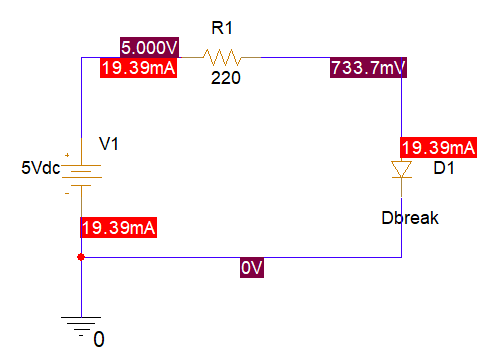
\includegraphics[width=0.8\linewidth]{graphics/ex1/f1.PNG}
    \end{subfigure}
    \hfill
    \begin{subfigure}{0.45\textwidth}
        \centering
        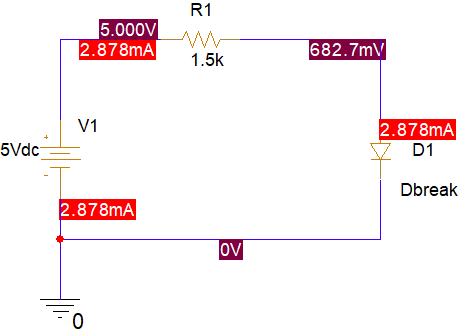
\includegraphics[width=0.8\linewidth]{graphics/ex1/f2.PNG}
    \end{subfigure}
    \caption{Kết quả mô phỏng trên PSpice}
    \label{fig:sidebyside}
\end{figure}

\subsection{So sánh}    

Trong phần này, các tính toán lý thuyết và mô phỏng PSpice được tóm tắt trong bảng bên dưới để so sánh sự khác biệt. Học sinh được yêu cầu điền tất cả thông tin vào bảng.

\begin{table}[h]
    \centering
    \begin{tabular}{@{}lcccccc@{}}
        \toprule
        & \multicolumn{3}{c}{\textbf{Theory}} & \multicolumn{3}{c}{\textbf{PSpice}} \\
        \cmidrule(rl{0.5cm}){2-4} \cmidrule(rl{0.5cm}){5-7}
        & \textbf{$V_R$} & \textbf{$V_D$} & \textbf{$I$} & \textbf{$V_R$} & \textbf{$V_D$} & \textbf{$I$} \\
        \midrule
        R = 220 Ohm  & 3.503 V & 1.497 V & 15.92 mA & 4.266 V & 0.734 V & 19.39 mA \\ 
        R = 1.5 K Ohm & 4.161 V & 0.839 V & 2.774 mA & 4.378 V & 0.622 V & 2.919 mA \\ 
        \bottomrule
    \end{tabular}
\end{table}

Theo Kết quả Bài tập trên, hãy đưa ra một số nhận xét về quan sát (giữa kết quả tính toán và kết quả mô phỏng):

Dựa vào kết quả trên, chúng ta có thể thấy rằng kết quả tính toán và kết quả mô phỏng có đôi chút khác biệt, điều này có thể được giải thích bởi điện trở bên trong diode, không phải là giá trị hằng số.